%=====================================================
\begin{frame}{2.2.5. Тип организации взаимодействия по обмену опытом}


\tiny

На диаграмме представлен сводный результат по вопросу Б24:
\bigskip

\begin{itemize}
\item [Б24] Обычные действия после посещения открытых и неподготовленных занятий. ``После посещения занятий  и мероприятий (открытых и неоткрытых)  в нашей образовательной организации  обычно:''
\end{itemize}

\begin{columns}
\begin{column}{0.4\textwidth} 
\centering
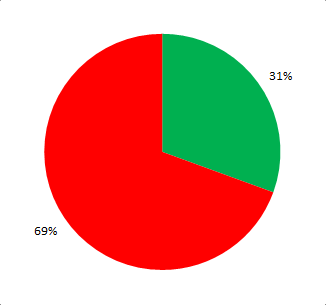
\includegraphics[width=4cm, height=4cm]{diag.png}
\end{column}
\begin{column}{0.6\textwidth} \begin{tabular}{l} 
 Занятие (мероприятие) обсуждается \\
один на один с преподавателем --- \valBBEansA\ (\valBBEansAp\%)  \\[0.5cm] 
Занятие (мероприятие)   анализируется \\
с администрацией ---   \valBBEansB\ (\valBBEansBp\%) \\[0.5cm]
Организуется групповое обсуждение \\
занятия (мероприятия) всеми \\
присутствовавшими на нем  --- \valBBEansC\ (\valBBEansCp\%) \\[0.5cm]
Ничего не происходит ---  \valBBEansD\ (\valBBEansDp\%) \\[0.5cm]
\end{tabular}
\end{column}
\end{columns}

\end{frame}


